\documentclass[border=2pt]{standalone}
\usepackage{tikz}\usetikzlibrary{arrows.meta,positioning,shapes.geometric,fit,calc}
\usepackage{newtxtext}
\renewcommand{\familydefault}{\sfdefault}
\begin{document}
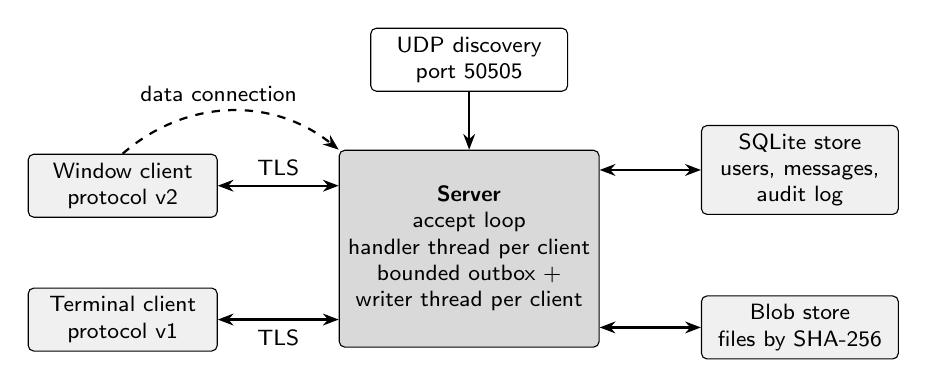
\begin{tikzpicture}[
  box/.style={draw, rounded corners=2pt, font=\footnotesize, align=center, minimum height=8mm, inner sep=3pt},
  arr/.style={{Stealth[length=2mm]}-{Stealth[length=2mm]}, thick},
  one/.style={-{Stealth[length=2mm]}, thick}
]
\node[box, fill=gray!12, minimum width=2.4cm] (gui) at (0,1.0) {Window client\\protocol v2};
\node[box, fill=gray!12, minimum width=2.4cm] (term) at (0,-0.7) {Terminal client\\protocol v1};
\node[box, fill=gray!30, minimum width=3.3cm, minimum height=2.5cm] (srv) at (4.4,0.2) {\textbf{Server}\\accept loop\\handler thread per client\\bounded outbox +\\writer thread per client};
\node[box, fill=gray!12, minimum width=2.5cm] (db) at (8.6,1.2) {SQLite store\\users, messages,\\audit log};
\node[box, fill=gray!12, minimum width=2.5cm] (blob) at (8.6,-0.8) {Blob store\\files by SHA-256};
\node[box, fill=white, minimum width=2.5cm] (udp) at (4.4,2.6) {UDP discovery\\port 50505};
\draw[arr] (gui)--node[above,font=\footnotesize]{TLS}(srv.west |- gui);
\draw[arr] (term)--node[below,font=\footnotesize]{TLS}(srv.west |- term);
\draw[arr] (srv.east |- db)--(db);
\draw[arr] (srv.east |- blob)--(blob);
\draw[one] (udp)--(srv);
\draw[one, dashed] (gui.north) to[bend left=40] node[above,font=\footnotesize,pos=0.45]{data connection} (srv.north west);
\end{tikzpicture}
\end{document}
